\documentclass{article} % This command is used to set the type of
% document you are working on such as an article, book, or presentation

\usepackage{geometry} % This package allows the editing of the page layout
\usepackage{amsmath}  % This package allows the use of a large range
% of mathematical formula, commands, and symbols
\usepackage{graphicx}  % This package allows the importing of images
\usepackage{
  minted,
  float,
  amsmath,      % Math Environments
  amssymb,      % Extended Symbols
  enumerate,        % Enumerate Environments
  graphicx,      % Include Images
  lastpage,      % Reference Lastpage
  multicol,      % Use Multi-columns
  multirow      % Use Multi-rows
}
\usepackage{amsmath}
\DeclareMathOperator*{\argmax}{arg\,max}
\DeclareMathOperator*{\argmin}{arg\,min}
\newcommand{\question}[2][]{
  \begin{flushleft}
    \textbf{Question #1}: \textit{#2}

\end{flushleft}}
\newcommand{\sol}{\textbf{Solution}:} %Use if you want a boldface solution line
\newcommand{\maketitletwo}[2][]{
  \begin{center}
    \Large{\textbf{Assignment #1}

    CS 4375} % Name of course here
    \vspace{5pt}

    \normalsize{N. Ohayon Rozanes  % Your name here

    \today}        % Change to due date if preferred
    \vspace{15pt}

\end{center}}
\begin{document}
\maketitletwo[5]  % Optional argument is assignment number
%Keep a blank space between maketitletwo and \question[1]

\question[1]{Nearest Neighbor Models}
\begin{enumerate}[(a)]
  \item The parameter $k$ has a direction correlation with the bias,
    and an inverse relation with variance. To see this, note that if
    the implementation does consider the point itself as a
    neighbor, then for $k=1$, each point is categorized as its own
    category, so the error is exactly $0$ (if the implementation does
      not use the point itself as a neighbor, the bias would still be
      relatively low if the $k$-NN assumption holds, which is that
    points close together are of the same class), and therefore the
    algorithm is unbiased. However, the algorithm will produce a
    classification with exactly as much variance as the data set. If,
    on the other hand, $k = N$, where $N$ is the number of samples in
    the data set, then every point will consider every other point in
    the classification, so every point will be categorized as the
    majority class in the data set, and therefore will have no
    variance at all, but will misclassify every sample which is in a
    minority class, leading to a high bias.
  \item
    \begin{itemize}
      \item $k$-NN is not robust to the presence of low correlation
        features, this is because each feature contributes an equal
        amount to the distance calculation. If two samples $X_n$ and
        $X_m$ share a class, but are very different from one another
        in a low correlation feature $x_j$, then $X_n$ will likely
        not be considered in the classification of $X_m$, and vice
        versa. Exactly how damaging a low correlation feature is to
        the model depends on the distribution of that feature, since
        a low variance feature will contribute about the same to the
        distances calculations, while a high variance feature will
        cause discrepancies like the one described above.
      \item For a similar reason to the above, dynamic ranges harm a
        $k$-NN model. The larger magnitude feature will dominate the
        distance calculation, so the algorithm will pick neighbors
        which are closer in that feature and mostly disregard the
        smaller magnitude features.
      \item As a computational consideration, a high dimensional
        feature set is not impactful since it only increases the
        computational complexity of the Euclidean metric, which is
        relatively efficient. However, distances become concentrated
        at higher dimensions, to see why this is true, consider that
        for the random vector of features $X = [X_1, X_2 \hdots X_n]$
        (for simplicity assume that each feature is drawn from i.i.d
        distributions) then by the law of large numbers:
        \[
          \frac{1}{n}\sum X_n^2  \to E[X_1^2]
        \]
        as $n \to \infty$, then clearly
        \[
          ||X||_2 \to \sqrt{nE[X_1^2]}
        \]
        $n \to \infty$, which is constant (the above manipulation is
          justified by the almost sure convergence that the strong
        law of large numbers gives). Because of this, in high
        dimensions, the distances between data points become less
        meaningful, and $k$-NN's assumption, that points close
        together should roughly be in the same category, breaks apart.
    \end{itemize}
  \item The code for the $k$-NN algorithm can be found in the
    appendix, testing on the iris data set led to a test accuracy of
    $0.9333$ for $k=1$, $0.97778$ for $k=5$ and $0.9556$ for $k=15$.
    Further, the plot of sepal width/length is shown along with
    categories for the various $k$'s. Note that, per standard
    implementation, the algorithm does not consider the point itself,
    leading to lackluster accuracy results for the case $k=1$. Still,
    the results roughly line up with what we're expecting, seeing as
    how at higher $k$, the accuracy begins to decrease, implying a higher bias.
    \begin{figure}[t]
      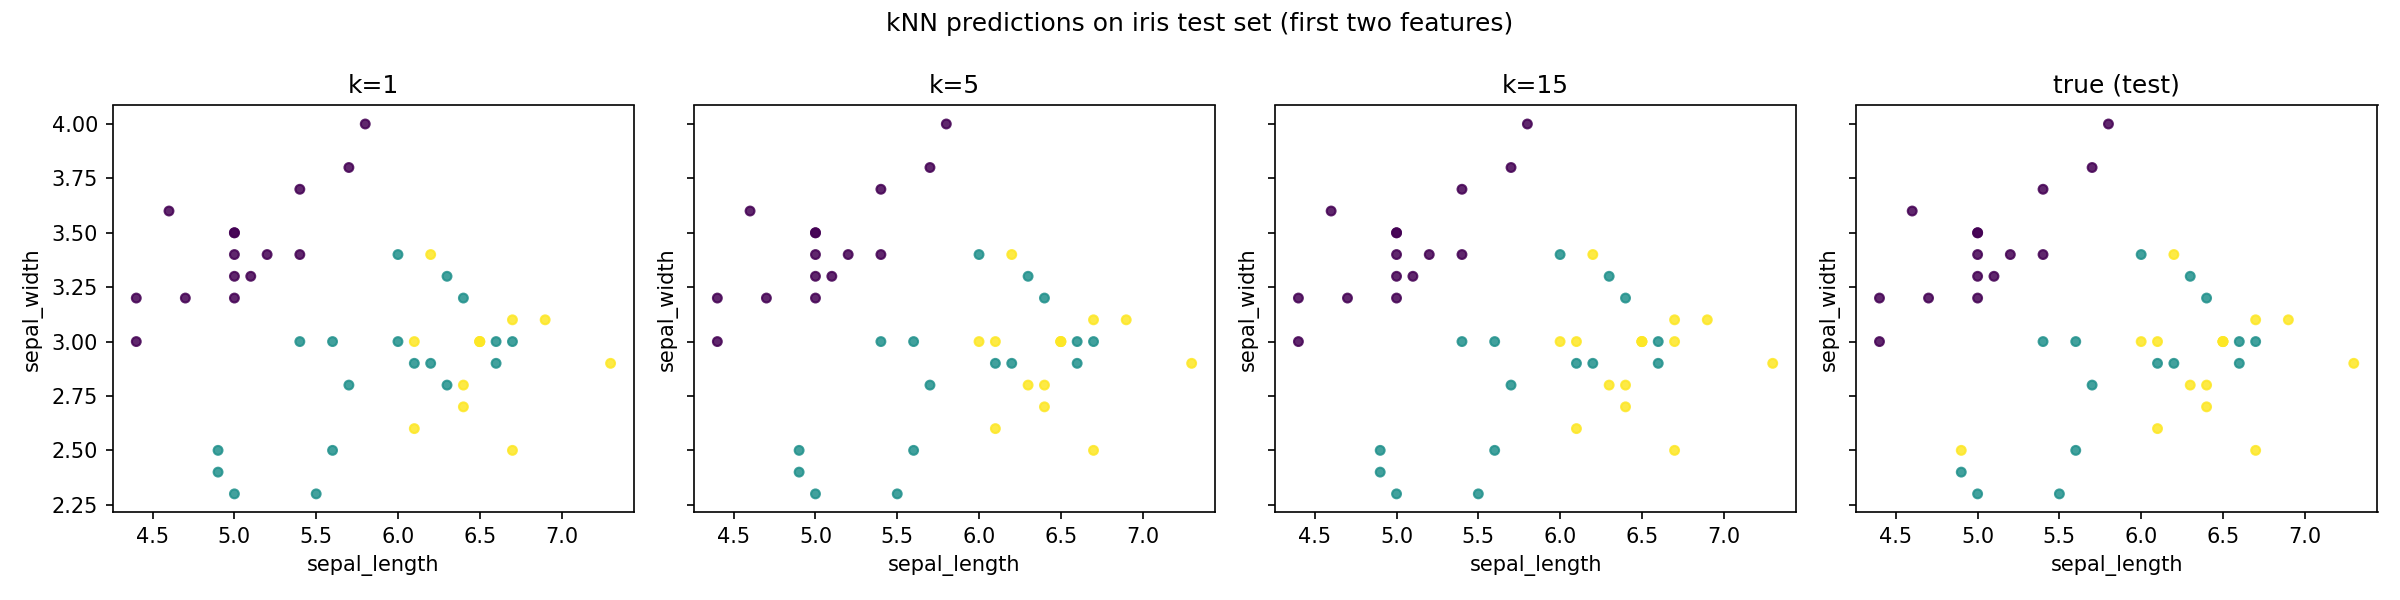
\includegraphics[scale=0.4]{knn_iris_k_plots.png}
      \caption{Fig. 1 k-NN classification of datasets at various k}
      \centering
    \end{figure}
\end{enumerate}

\question[2]{Decision Trees}
\begin{enumerate}[(a)]
  \item For a feature split $X$, and a label $Y$ the information gain
    that the split $X$ would gain is given by:
    \[
      \text{IG}(X) = H(Y) - H(Y|X)
    \]
    Where $H$ is the entropy function. We can interpret this
    intuitively as being the amount of uncertainty left in the
    label $Y$ after making the partition $X$. $H(Y)$ is the amount of
    uncertainty up to this point in the tree, $H(Y|X)$ represents the
    amount of uncertainty given that we split on $X$, thus their
    subtraction is the reduction of uncertainty (gain in certainty)
    caused by $X$. To further illustrate the behavior of the
    information gain function, consider that, if the
    label is independent of the split, then $H(Y|X) = H(Y)$ so
    $\text{IG}(X) = 0$, as expected, since we would gain no new
    information if the split is independent of the feature.
  \item Results from \texttt{code/descision\_tree.py}:
    \begin{verbatim}
x2 < 0.0929 (level=0, pred=0)
  x2 < -0.4388 (level=1, pred=0)
    x2 < -1.0288 (level=2, pred=0)
    x1 < 0.0404 (level=2, pred=0)
  x2 < 0.4389 (level=1, pred=1)
    x1 < -0.6443 (level=2, pred=0)
    x1 < -2.3047 (level=2, pred=1)
MSE: 0.1800
    \end{verbatim}
    A scatterplot of the generated synthetic data is pictured in
    Figure 2. All code is in the appendix. Notably, to get the MSE to
    be nonzero required a little bit of manual working of the data,
    adding additional noise to the random generation as well as
    creating blocks where the two classes would overlap more heavily.
    \begin{figure}[H]
      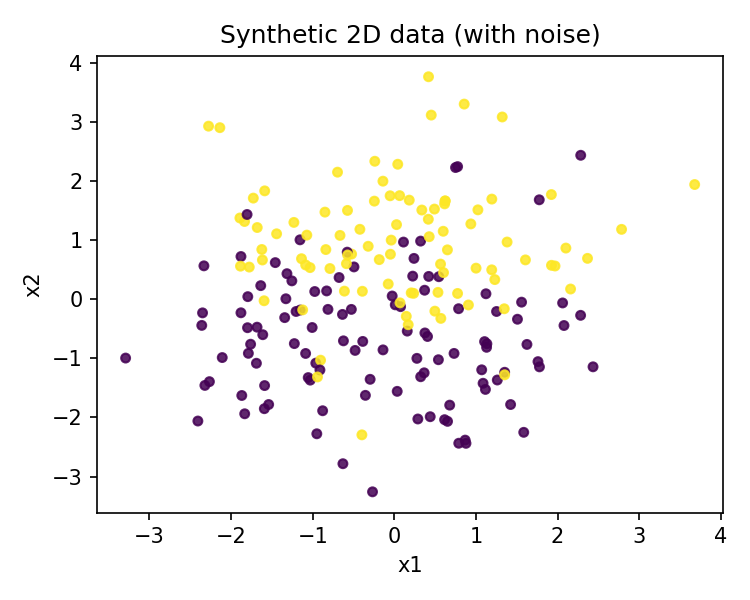
\includegraphics[scale=0.5]{decision_tree_data.png}
      \centering
      \caption{Fig. 2 Synthetic 2D data (with noise) for decision tree}
    \end{figure}
    The bulk of the work for the decision tree was in calculating the
    optimal split, which was done in this function:
    \begin{minted}{python}
    def find_split_ig(df, label):
    if len(df) == 0:
        return None, None, None
    X = df.drop(columns=[label])
    candidates = []
    for col in X.columns:
        sorted_vals = np.sort(df[col].to_numpy())
        midpoints = [(a + b) / 2 for a, b in zip(sorted_vals, sorted_vals[1:])]
        if not midpoints:
            continue
        ig = []
        for point in midpoints:
            left_mask = df[col] < point
            right_mask = ~left_mask
            p_left = (left_mask).mean()
            p_right = 1.0 - p_left
            p_y_left = df.loc[left_mask, label].value_counts(normalize=True)
            p_y_right = df.loc[right_mask, label].value_counts(normalize=True)
            h_left = -(p_y_left * np.log2(p_y_left)).sum()
            h_right = -(p_y_right * np.log2(p_y_right)).sum()
            h_y_x = p_left * h_left + p_right * h_right
            p_y = (df[label]).value_counts(normalize=True)
            h_y = -(p_y * np.log2(p_y)).sum()
            ig.append(h_y - h_y_x)
        best_idx = int(np.argmax(ig))
        candidates.append((midpoints[best_idx], ig[best_idx], col))
    if not candidates:
        return None, None, None
    return max(candidates, key=lambda item: item[1])
    \end{minted}
    On simpler datasets, there would sometimes not be enough points
    where a split would be necessary, hence the None checking.
\end{enumerate}
\question[3]{Bayes' Rule}
\begin{enumerate}[(a)]
  \item For random variables $X, B$, Bayes' rule states that
    \[
      P(Y|X) = \frac{P(X|Y)P(Y)}{P(X)}
    \]
    In a supervised context, take each class to be a random variable
    $Y_i$, and $X$ to be a random vector of features, then we use
    Bayes' rule to calculate the probability of each class given the
    data:
    \[
      P(Y_i|X) = \frac{P(X|Y_i)P(Y_i)}{P(X)}
    \]
    Since $X$ is a random vector $P(X) = P(x_1)P(x_2)\hdots P(x_n)$
    and $P(X|Y_i) = P(x_1|Y_i)P(x_2|Y_i)\hdots P(x_n|Y_i)$. Thus the
    formula becomes:
    \[
      P(Y_i|X) = \frac{P(x_1|Y_i)P(x_2|Y_i)\hdots
      P(x_n|Y_i)P(Y_i)}{P(x_1)P(x_2)\hdots P(x_n)}
    \]
    Since, the denominator is constant across classes of $Y_i$, we
    can ignore it, so the classification rule which maximizes the
    probability of correct classification is
    \[
      \text{argmax}_i \left( P(Y_i)\prod_n^N P(x_n|Y_i)\right)
    \]
    Often, we compute the prior and conditional probabilities from a
    frequentist approximation of data. But sometimes the prior
    distribution (the distribution of labels) is known ahead of time.
  \item Suppose that $Y \sim \text{Beta}(2,2)$ and we observe $8$
    tosses with $6$ heads and $2$ tails which we denote as event $x$,
    then consider that a coin flip follows a Bernoulli distribution
    with parameter $Y$ so the multiple flips follow a binomial
    distribution. Thus, by Bayes' theorem, the posterior is given as
    \begin{align*}
      p(Y | x) = \frac{p(x|Y)}{p(x)}p(Y) &=
      \frac{\binom{8}{6}Y^{6}(1-Y)^{2}}{p(x)}\frac{1}{B(2,2)}Y^{2-1}(1-Y)^{2-1}\\
      &= \frac{\binom{8}{6}}{B(2,2)\,p(x)}Y^{7}(1-Y)^{3}
      = \frac{1}{B(8,4)}Y^{7}(1-Y)^{3}
    \end{align*}
    The last step is justified since $Y^7(1-Y)^{3}$ is an
    unnormalized $\text{Beta}(8,4)$ distribution, thus the constant
    factor before it must be $\frac{1}{B(8,4)}$; therefore,
    \[
      p(Y|x)\sim \text{Beta}{(8,4)}
    \]

\end{enumerate}
\question[4]{Naive Bayes}
\begin{enumerate}[(a)]
  \item
    \[
      P(\text{Spam}) = \frac{40 + 25 + 30 + 5}{40 + 25 + 30 + 5 + 5 +
      15 + 20 + 60} = \frac{100}{200} = \frac{1}{2}
    \]
    And
    \[
      P(\text{Not Spam}) = 1 - P(\text{Spam}) = \frac{1}{2}
    \]
  \item
    \begin{align*}
      P(\text{Spam}|\text{win, free}) &\propto
      P(\text{spam})P(\text{win}|\text{Spam})P(\text{free}|\text{Spam})
      = \frac{1}{2}\frac{65}{100}\frac{70}{100} = 0.2275\\
      P(\text{Not Spam}|\text{win, free}) &\propto
      P(\text{Not Spam})P(\text{win}|\text{Not
      Spam})P(\text{free}|\text{Not Spam})
      = \frac{1}{2}\frac{20}{100}\frac{25}{100} = 0.025
    \end{align*}
    Thus, we predict that an email containing the words win and free
    is a spam email.
  \item Code is in the appendix, the calculation matches.
\end{enumerate}
\question[5]{Logistic Regression}
\begin{enumerate}[(a)]
  \item The hypothesis function of the logistic function, for $x
    \in \mathbb{R}^n$, and $y = \{0,1\} $
    \[
      p(Y = 1| x) = p_{w,b}(x) = \frac{1}{1+e^{-(b + w^T x)}}
    \]
    The sigmoid function is used since it maps from the feature space
    in $\mathbb{R}^n$ to a value which ranges from $[0, 1]$, which we
    interpret as a probability. Essentially, the sigmoid function
    allows us to learn (regress) a probability of a label, given some
    data corresponding to it. It follows immediately that
    \[
      p(Y = 0 | x) = 1  - P(Y = 1 | x) = 1 - p_{w,b}(x)
    \]
    It's easy to see that $Y | x \sim \text{Bern}(p_{w,b}(x))$, so we have that
    \[
      p(Y|x) = p_{w,b}(x)^Y(1 - p_{w,b}(x))^{(1-Y)}
    \]
  \item Under MLE, we seek to maximize the likelihood function with
    respect to parameters $w, b$ which is given by:
    \[
      L = \prod_i p(y_i | x_i, w, b)
    \]
    Consider, that from the assumptions, we have that
    Equivalently, we maximize the log likelihood function, using the
    condition probability from the last step, we get that:
    \begin{align*}
      l &= \ln \prod_i p(y_i | x_i, w,b) \\
      &= \sum_i \ln p(y_i | x_i, w, b) \\
      &= \sum_i \ln p_{w,b}(x_i)^{y_i}(1 - p_{w,b}(x_i))^{(1-y_i)} \\
      &= \sum_i y_i\ln p_{w,b}(x_i) + (1-y_i)\ln(1-p_{w,b}(x_i)) \\
      &= \sum_i \left[y_i\ln \frac{1}{1+e^{-(b+w^T x_i)}} + (1-y_i)\ln
      \frac{e^{-(b+w^T x_i)}}{1+e^{-(b+w^T x_i)}}\right] \\
      &= \sum_i \left[y_i(b+w^T x_i) - \ln(1+e^{b+w^T x_i})\right]
    \end{align*}
    Taking partial derivatives, we obtain:
    \begin{align*}
      \frac{\partial l}{\partial w} &= \sum_i \left[y_i -
      \frac{1}{1+e^{-(b+w^T x_i)}}\right] x_i
      = \sum_i (y_i - p_{w,b}(x_i))x_i \\
      \frac{\partial l}{\partial b} &= \sum_i \left[y_i -
      \frac{1}{1+e^{-(b+w^T x_i)}}\right]
      = \sum_i (y_i - p_{w,b}(x_i))
    \end{align*}
  \item Decision boundary and plot from \texttt{code/logistic.py}:
    \begin{verbatim}
Decision boundary: -3.0857 x1 + 6.6124 x2 + -1.1803 = 0
    \end{verbatim}
    \begin{figure}[H]
      \centering
      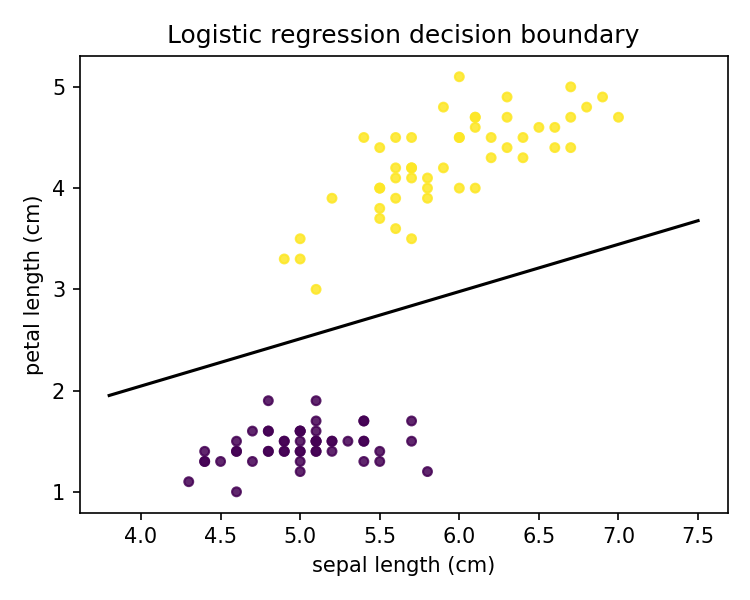
\includegraphics[scale=0.5]{logistic_boundary.png}
      \caption{Fig. 3 Logistic regression decision boundary (iris,
      two features)}
    \end{figure}
\end{enumerate}
\appendix
\section*{Appendix}
\subsection*{Question 1: Nearest Neighbor Models}
\inputminted{python}{code/knn.py}
\subsection*{Question 2: Decision Trees}
\inputminted{python}{code/descision_tree.py}
\subsection*{Question 4: Naive Bayes}
\inputminted{python}{code/naive_bayes.py}
\subsection*{Question 5: Logistic Regression}
\inputminted{python}{code/logistic.py}
\end{document}
